\section{Sequenzen}
    \subsection{Neue Zeiterfassung}
        Eine neue Zeiterfassung wird hinzugefügt.
        Dies kann entweder durch Übergabe von Start- und Endzeit oder durch das Starten und spätere Stoppen eines Timers geschehen.
        Falls der Stundenzettel für den entsprechenden Monat noch nicht existiert wird er erstellt.
        Nur Proletarier und Supervisor dürfen diese Aktion durchführen.
        Außerdem können nur Zeiterfassungen für Monate hinzugefügt werden, für die der Stundenzettel unlocked ist oder noch nicht existiert.\\

        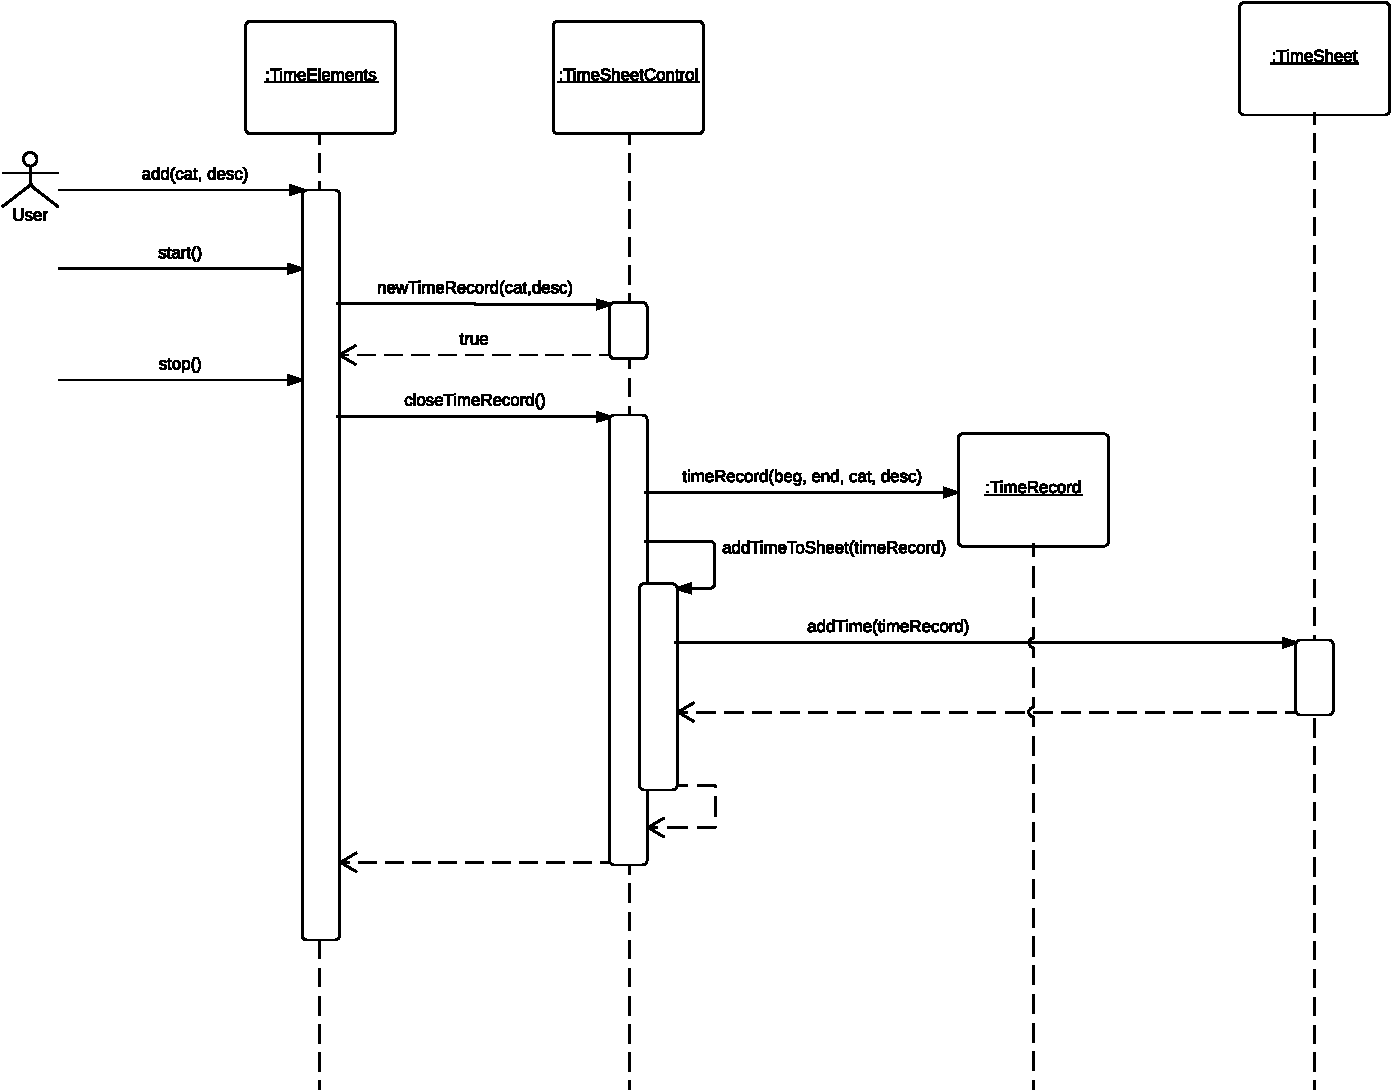
\includegraphics[width=\linewidth]{Diagramms/sequenzes/new_Time_record.pdf}

    \newpage
    \subsection{Login Sequenz}
        Ein User loggt sich ein.
        Falls als Authentifizierung LDAP statt Local ausgewählt ist, wird die Anfrage von LoginView stattdessen an den LDAP-Server weitergeleitet.
        Nur nicht eingeloggte User können diese Aktion durchführen.
        Für diese ist dies die einzige erlaubte Aktion.\\

        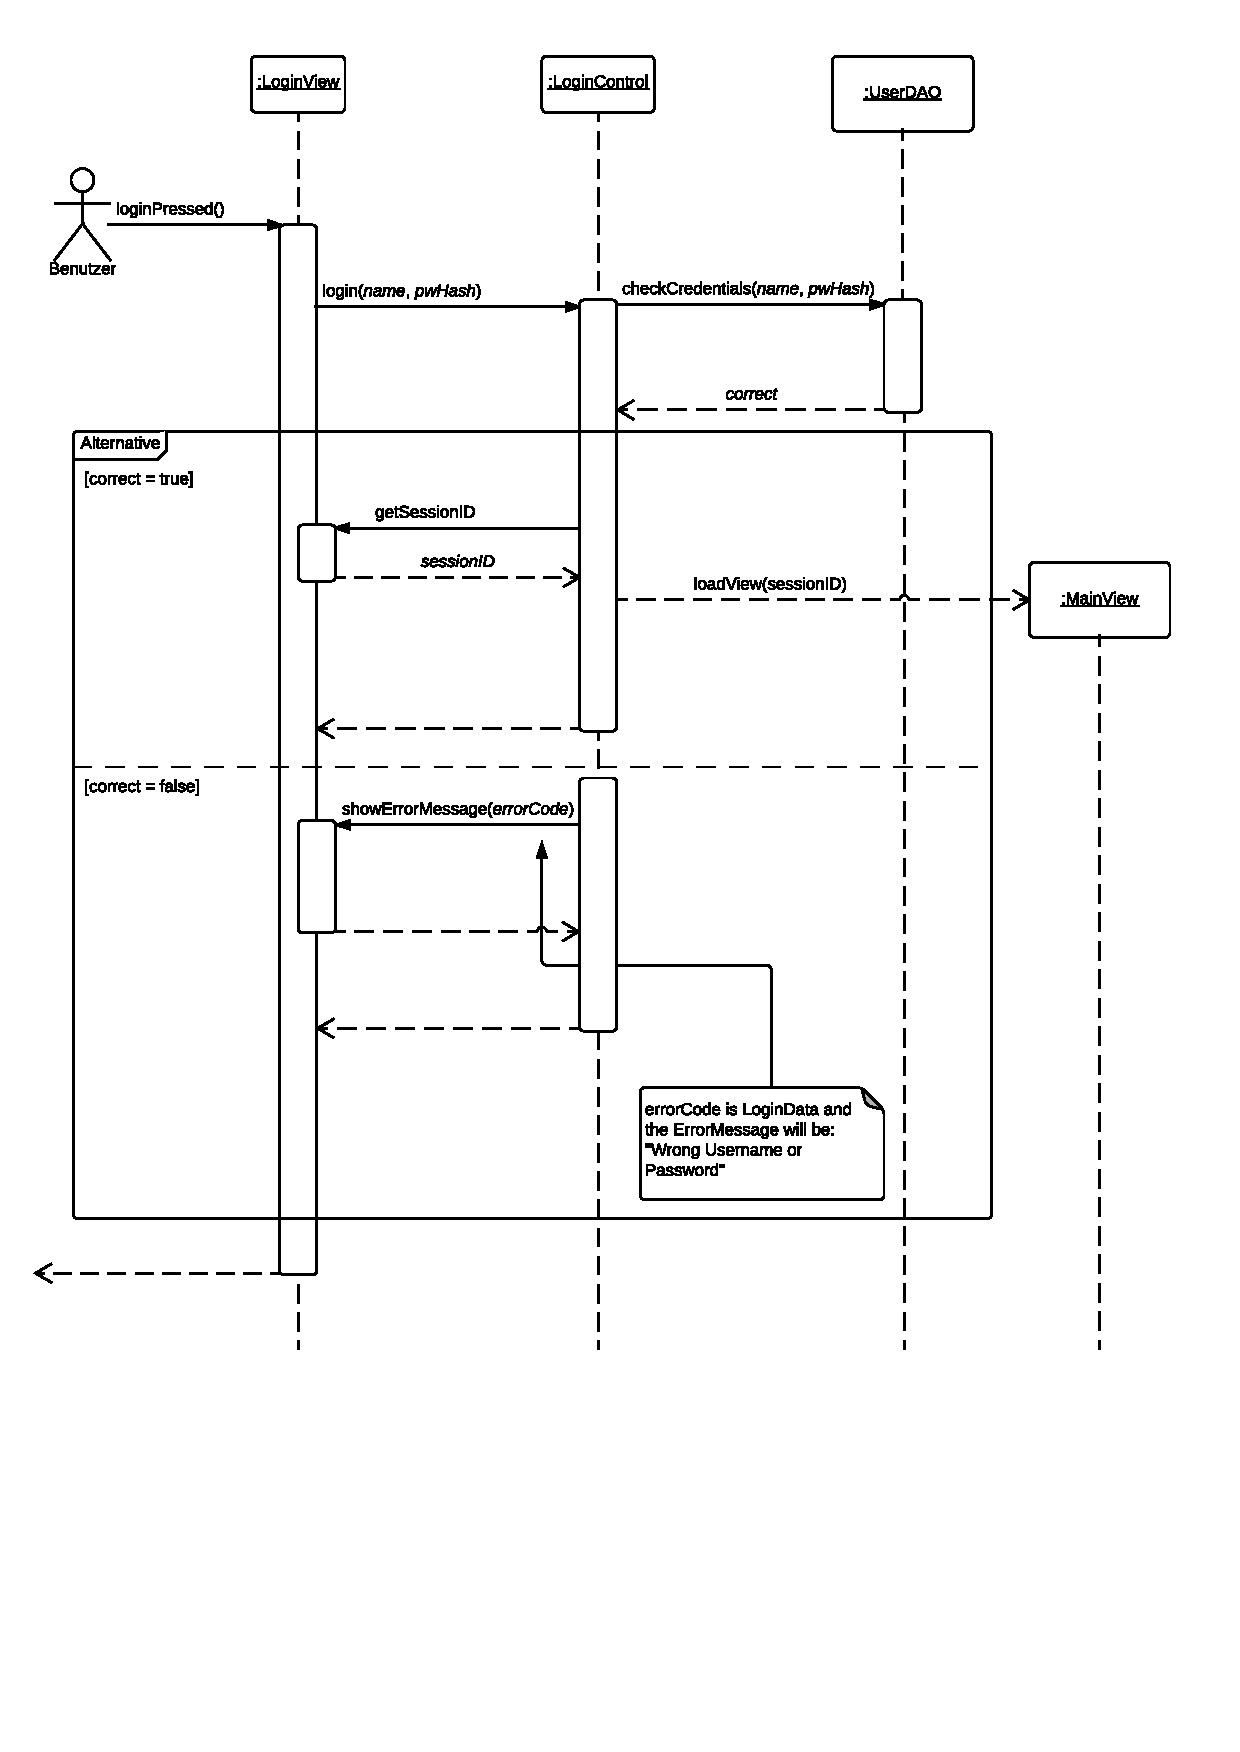
\includegraphics[width=\linewidth]{Diagramms/sequenzes/login.pdf}

    \newpage
    \subsection{Alle Stundenzettel der Gruppenmitglieder einsehen}
        Ein Supervisor lässt sich die Stundenzettel eines beliebigen Monats von allen von ihm betreuten Proletariern anzeigen.
        Supervisor können sich die Stundenzettel eines Monats von allen oder alle Stundenzettel eines von ihnen betreuten Proletariers anzeigen lassen.
        Administratoren können sich die Stundenzettel eines Monats aller Proletarier, nur aller von einem Supervisor betreuten Proletarier oder alle Stundenzettel eines Proletariers anzeigen lassen.
        Proletarier können diese Aktion nicht durchführen.\\

        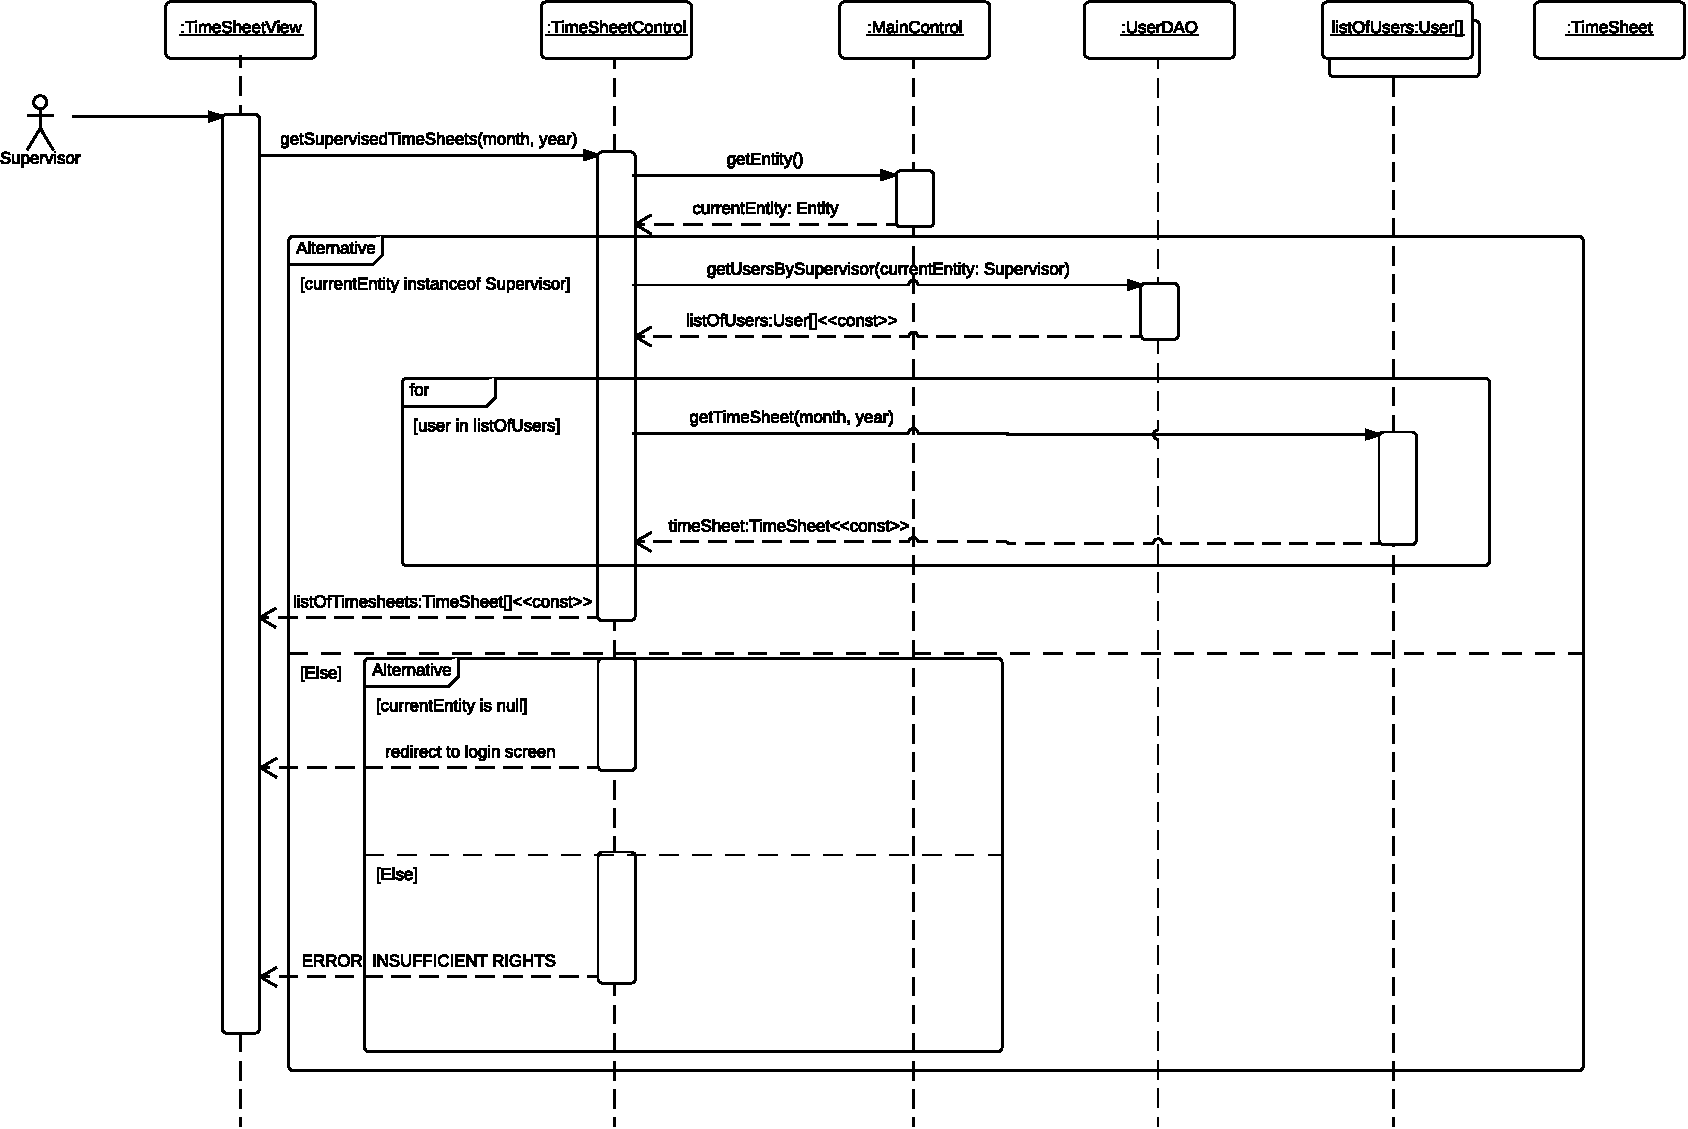
\includegraphics[width=\linewidth]{Diagramms/sequenzes/timesheets_of_all_supervised.pdf}

    \newpage
    \subsection{Aktuellen Stundenzettel einsehen}
        Ein Supervisor lässt sich den eigenen Stundenzettel des aktuellen Monats und die dazugehörigen Zeiterfassungen anzeigen.
        Diese Aktion kann für einen beliebigen Monat durchgeführt werden, solange ein Stundenzettel dafür existiert.
        Diese Aktion kann von Proletariern und Supervisorn durchgeführt werden.\\

        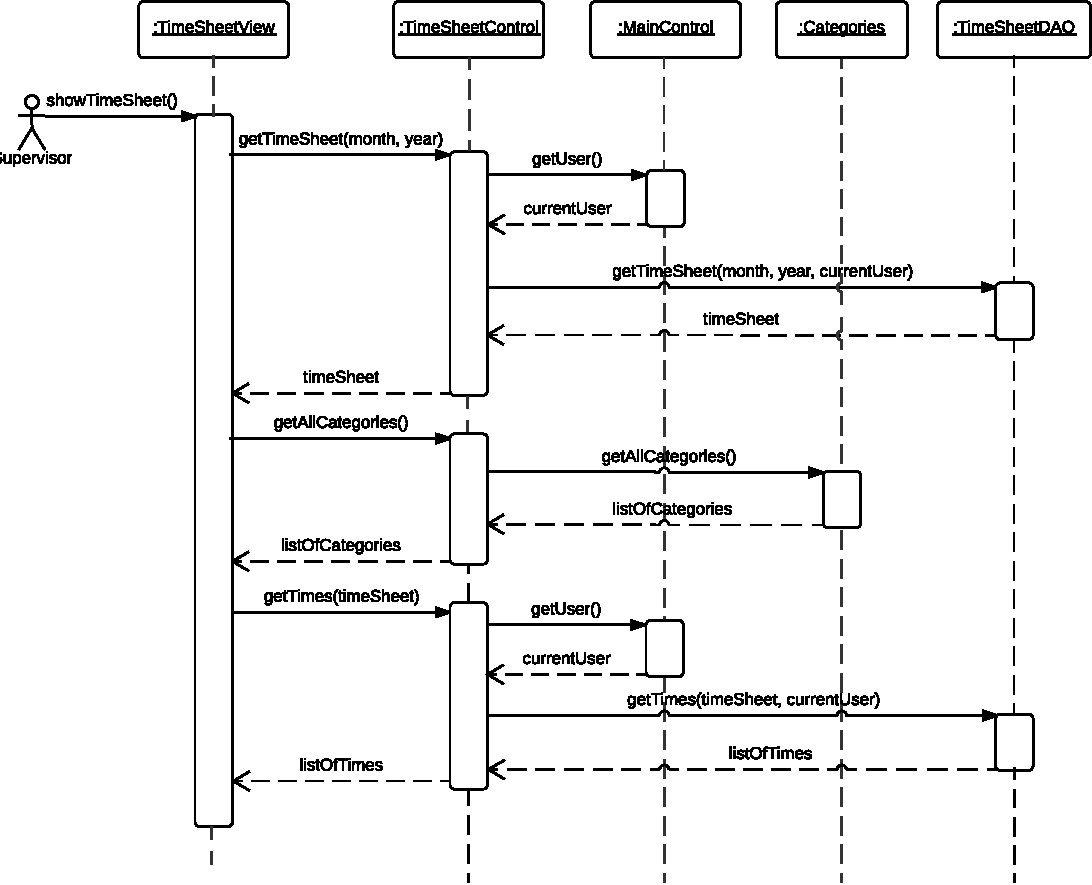
\includegraphics[width=\linewidth]{Diagramms/sequenzes/current_timesheet.pdf}

    \newpage
    \subsection{Stundenzettel abgeben}
        Ein Proletarier gibt seinen fertigen Stundenzettel ab.
        Dabei wird der Stundenzettel auf Fehler oder ähnliches überprüft und dann auf locked gesetzt.
        Dabei wird der Betreuer per Nachricht darüber informiert, damit dieser den Stundenzettel überprüfen kann.
        Diese Aktion kann von Proletariern und Supervisern ausgeführt werden.
        Superviser können außerdem Stundenzettel der von ihnen betreuten Proletarier von locked auf unlocked bzw. checked setzen.\\

        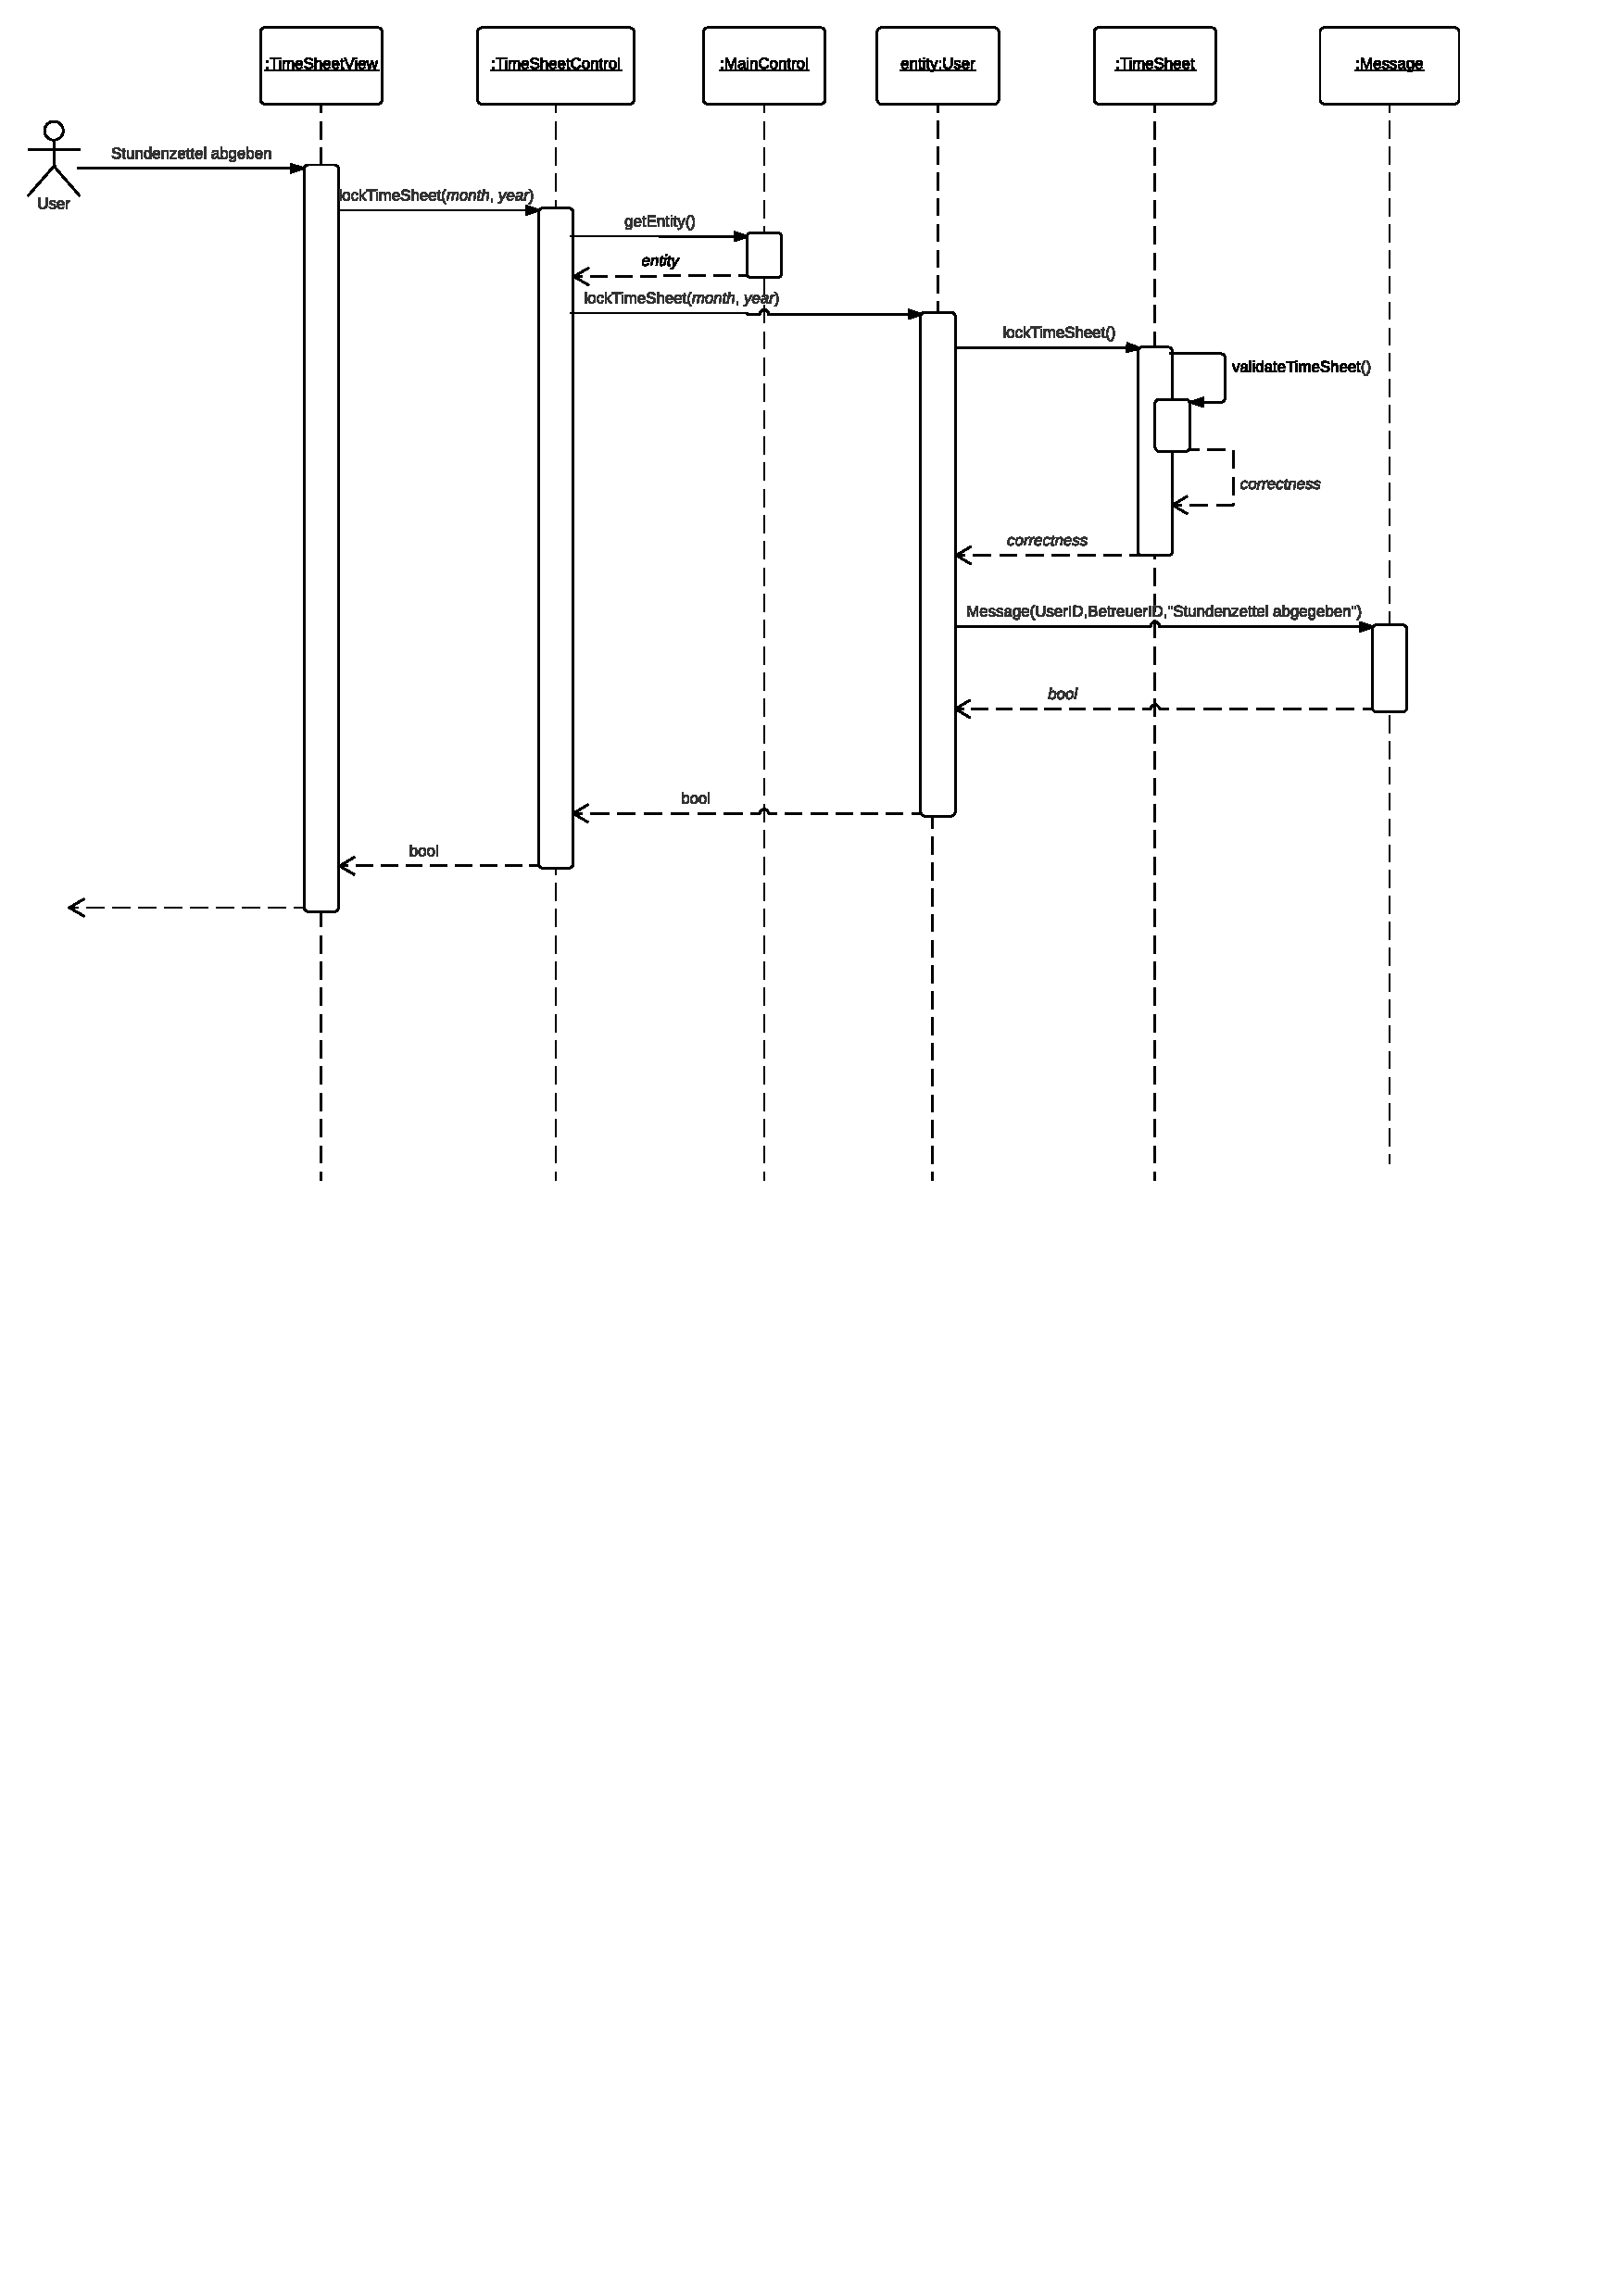
\includegraphics[width=\linewidth]{Diagramms/sequenzes/send_in_timesheet.pdf}

    \newpage
    \subsection{Benutzer anlegen}
        Ein neuer User wird angelegt.
        Falls LDAP zur Authentifizierung genutzt wird, muss kein Passwort angegeben werden.
        Falls ein Administrator angelegt wird, muss name, supervisor und hoursPerMonth nicht angegeben werden.
        Falls ein Supervisor angelegt wird, muss supervisor nicht angegeben werden.
        Diese Aktion kann nur von Administratoren ausgeführt werden.\\

        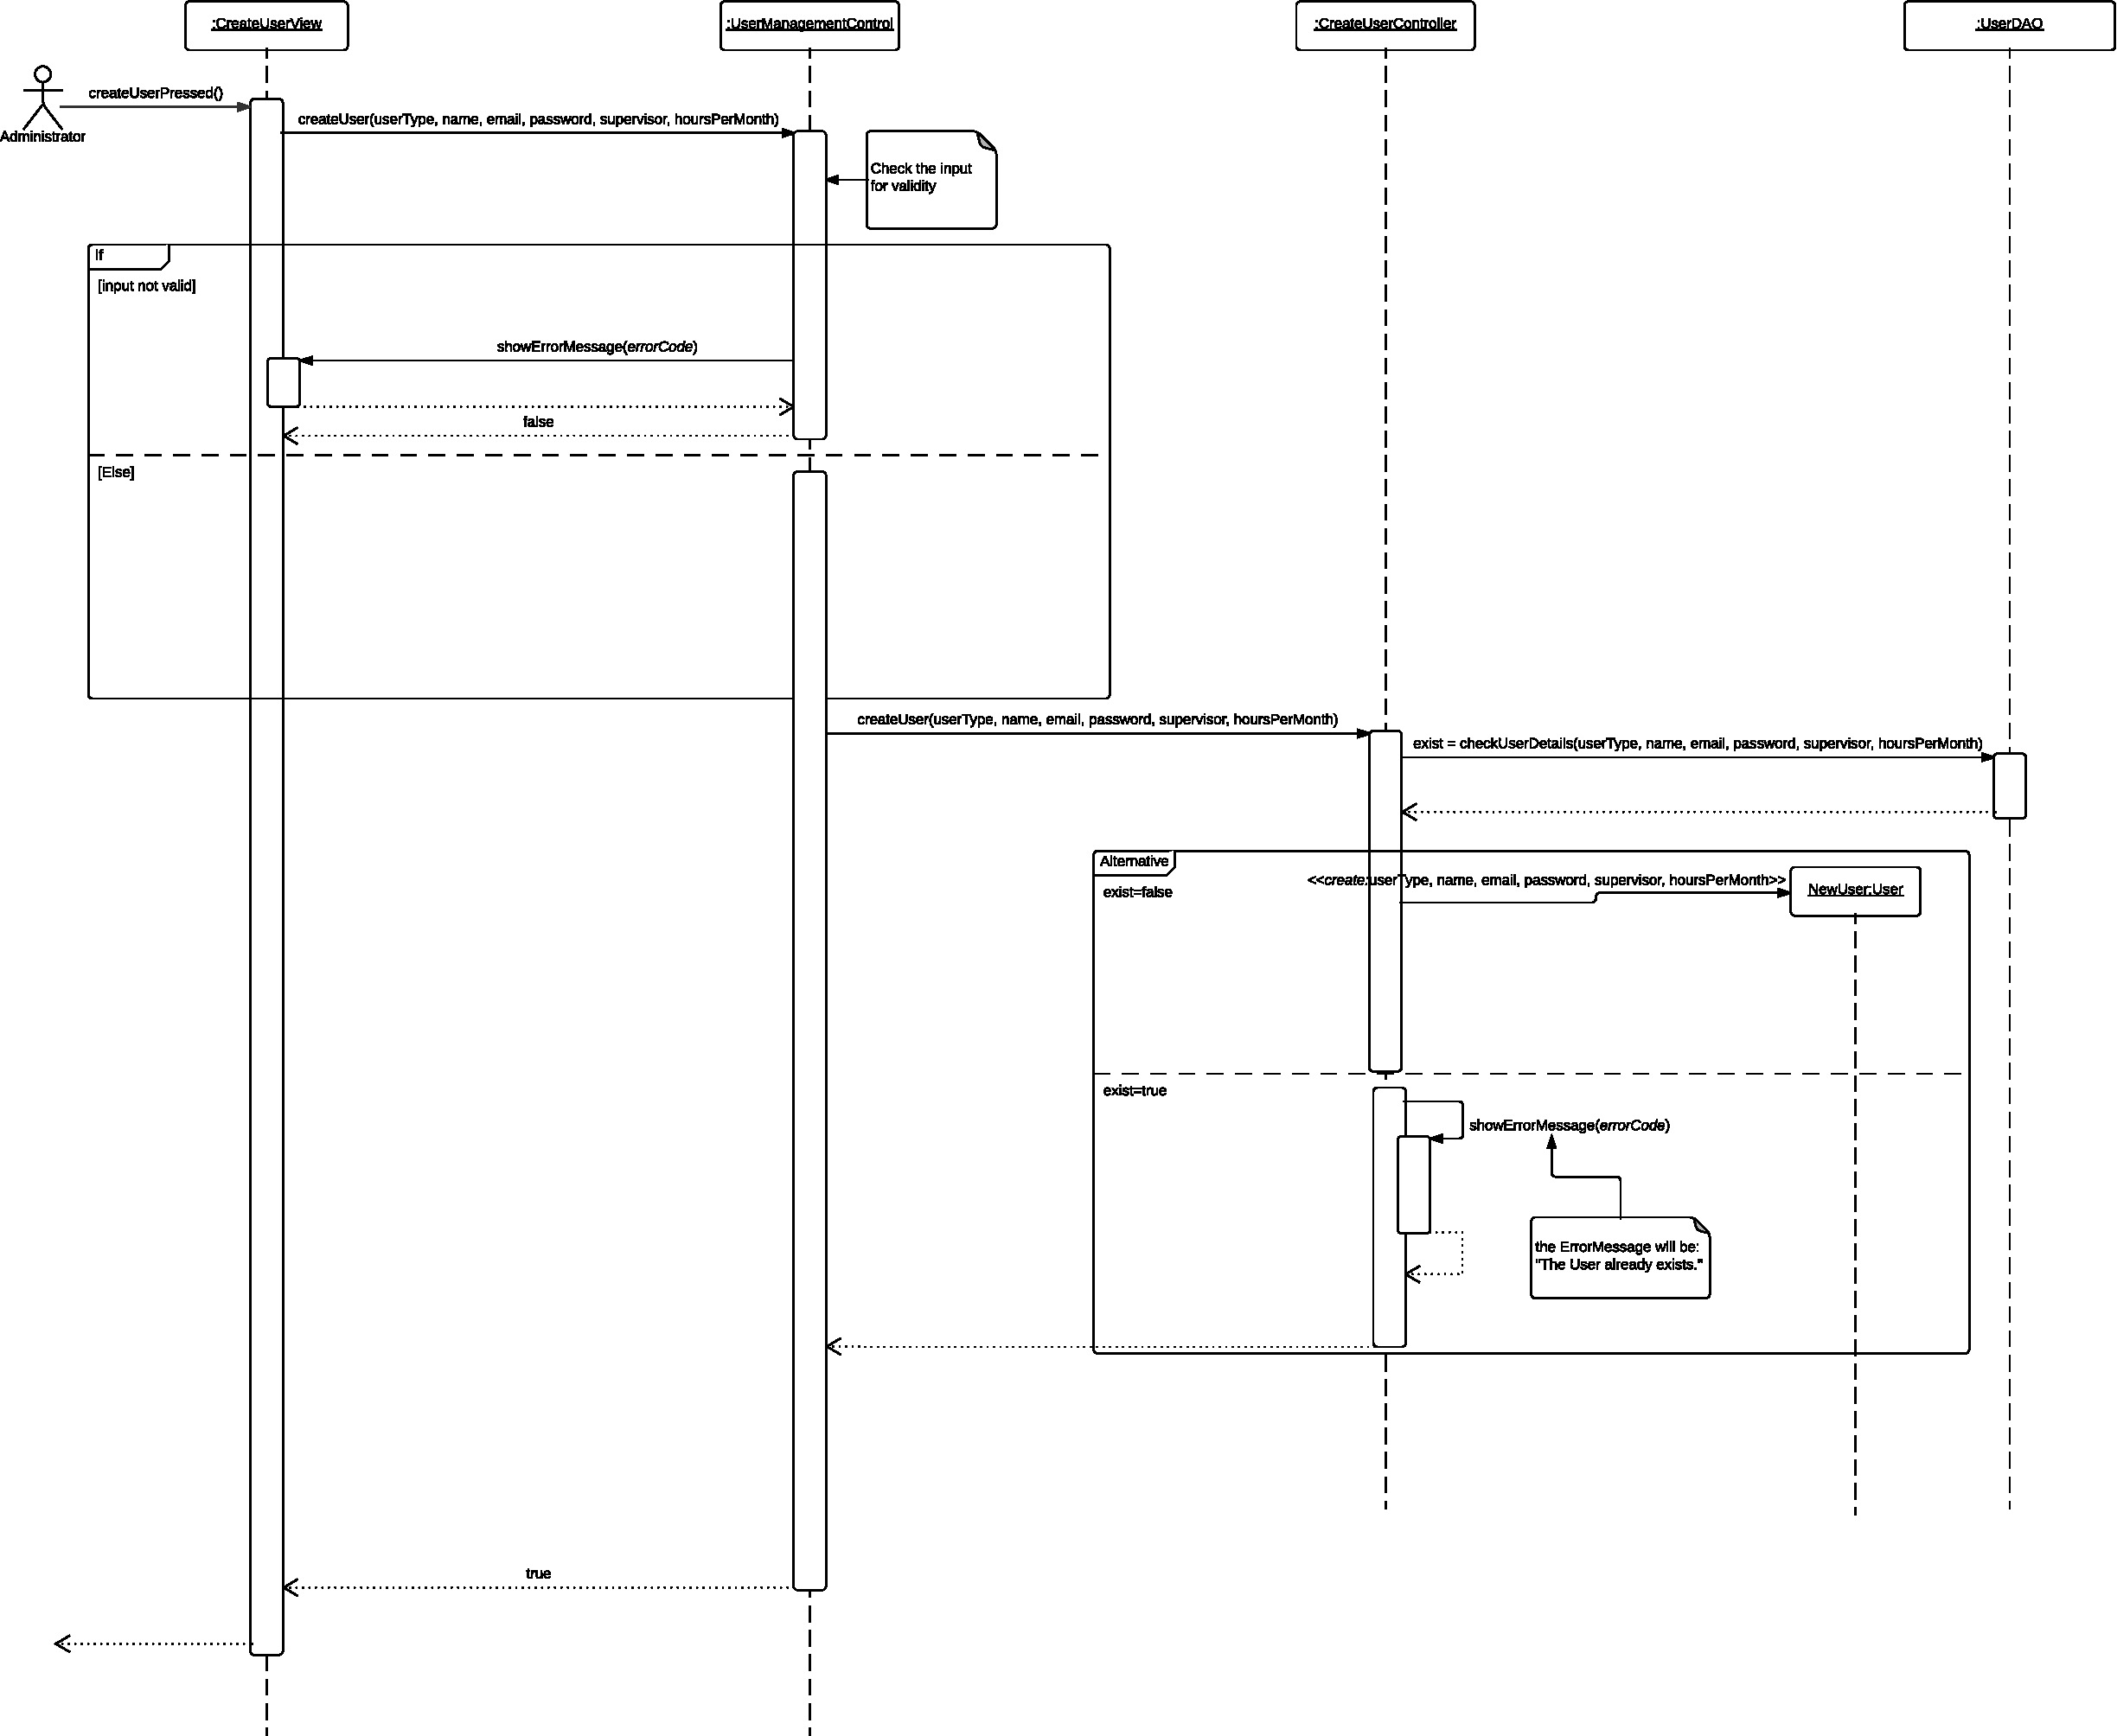
\includegraphics[width=\linewidth]{Diagramms/sequenzes/create_user.pdf}

    \newpage
    \subsection{Nachrichten verschicken}
        Eine Nachricht wird von einem User an einen anderen User verschickt.\\

        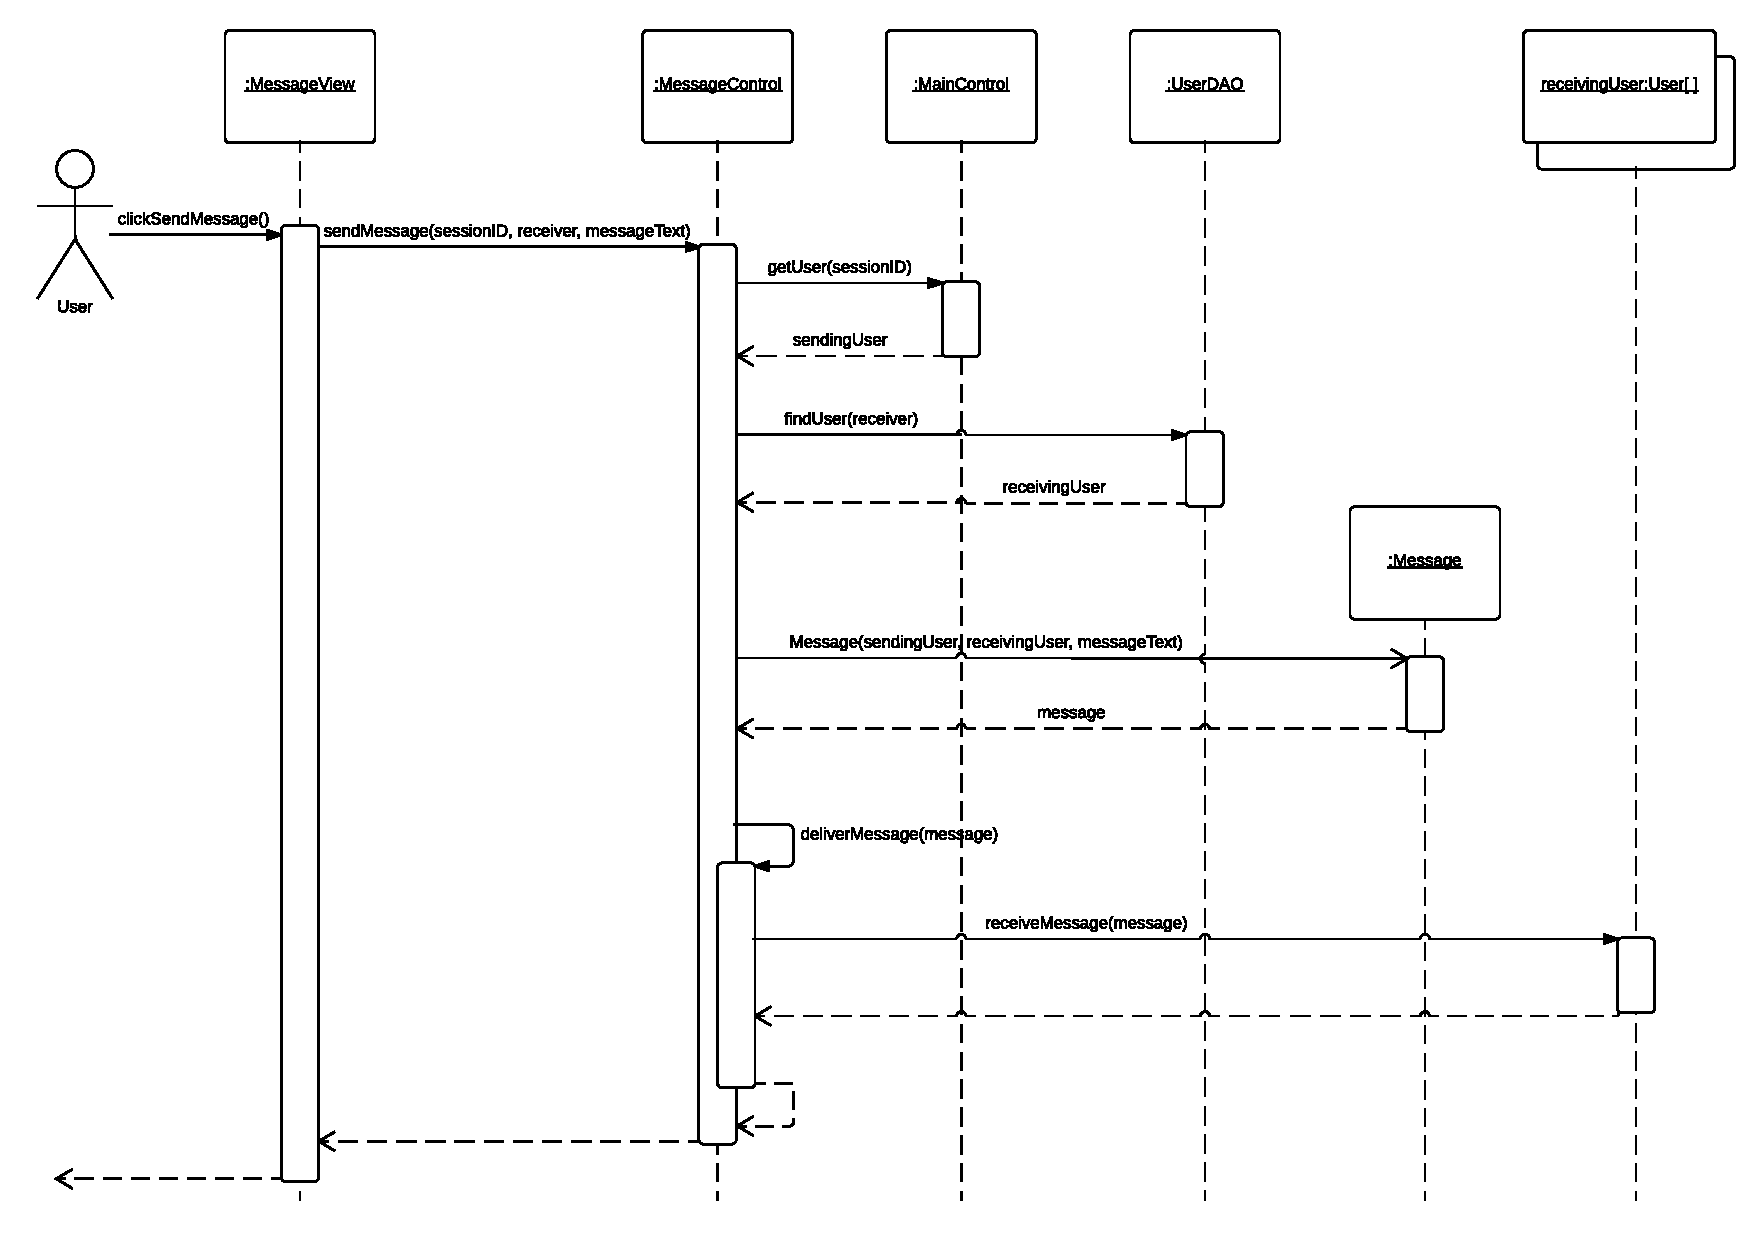
\includegraphics[width=\linewidth]{Diagramms/sequenzes/message_delivery.pdf}

    \newpage
    \subsection{Administrator exportiert alle Stundenzettel}
        Ein Administrator exportiert alle Stundenzettel eines Monats als ein zusammenhängendes pdf die den Status checked haben.
        Administratoren können zudem alle Stundenzettel eines Monats unabhängig vom Status, einen oder alle Stundenzettel eines Proletariers exportieren.
        Proletarier können einen oder alle ihre Stundenzettel exportieren.
        Supervisor können von ihren betreuten Proletariern alle Stundenzettel eines Monats die checked sind oder unabhängig von ihrem status exportieren.
        Zudem können sie einen oder alle Stundenzettel eines von ihnen betreuten Proletariers exportieren.\\

        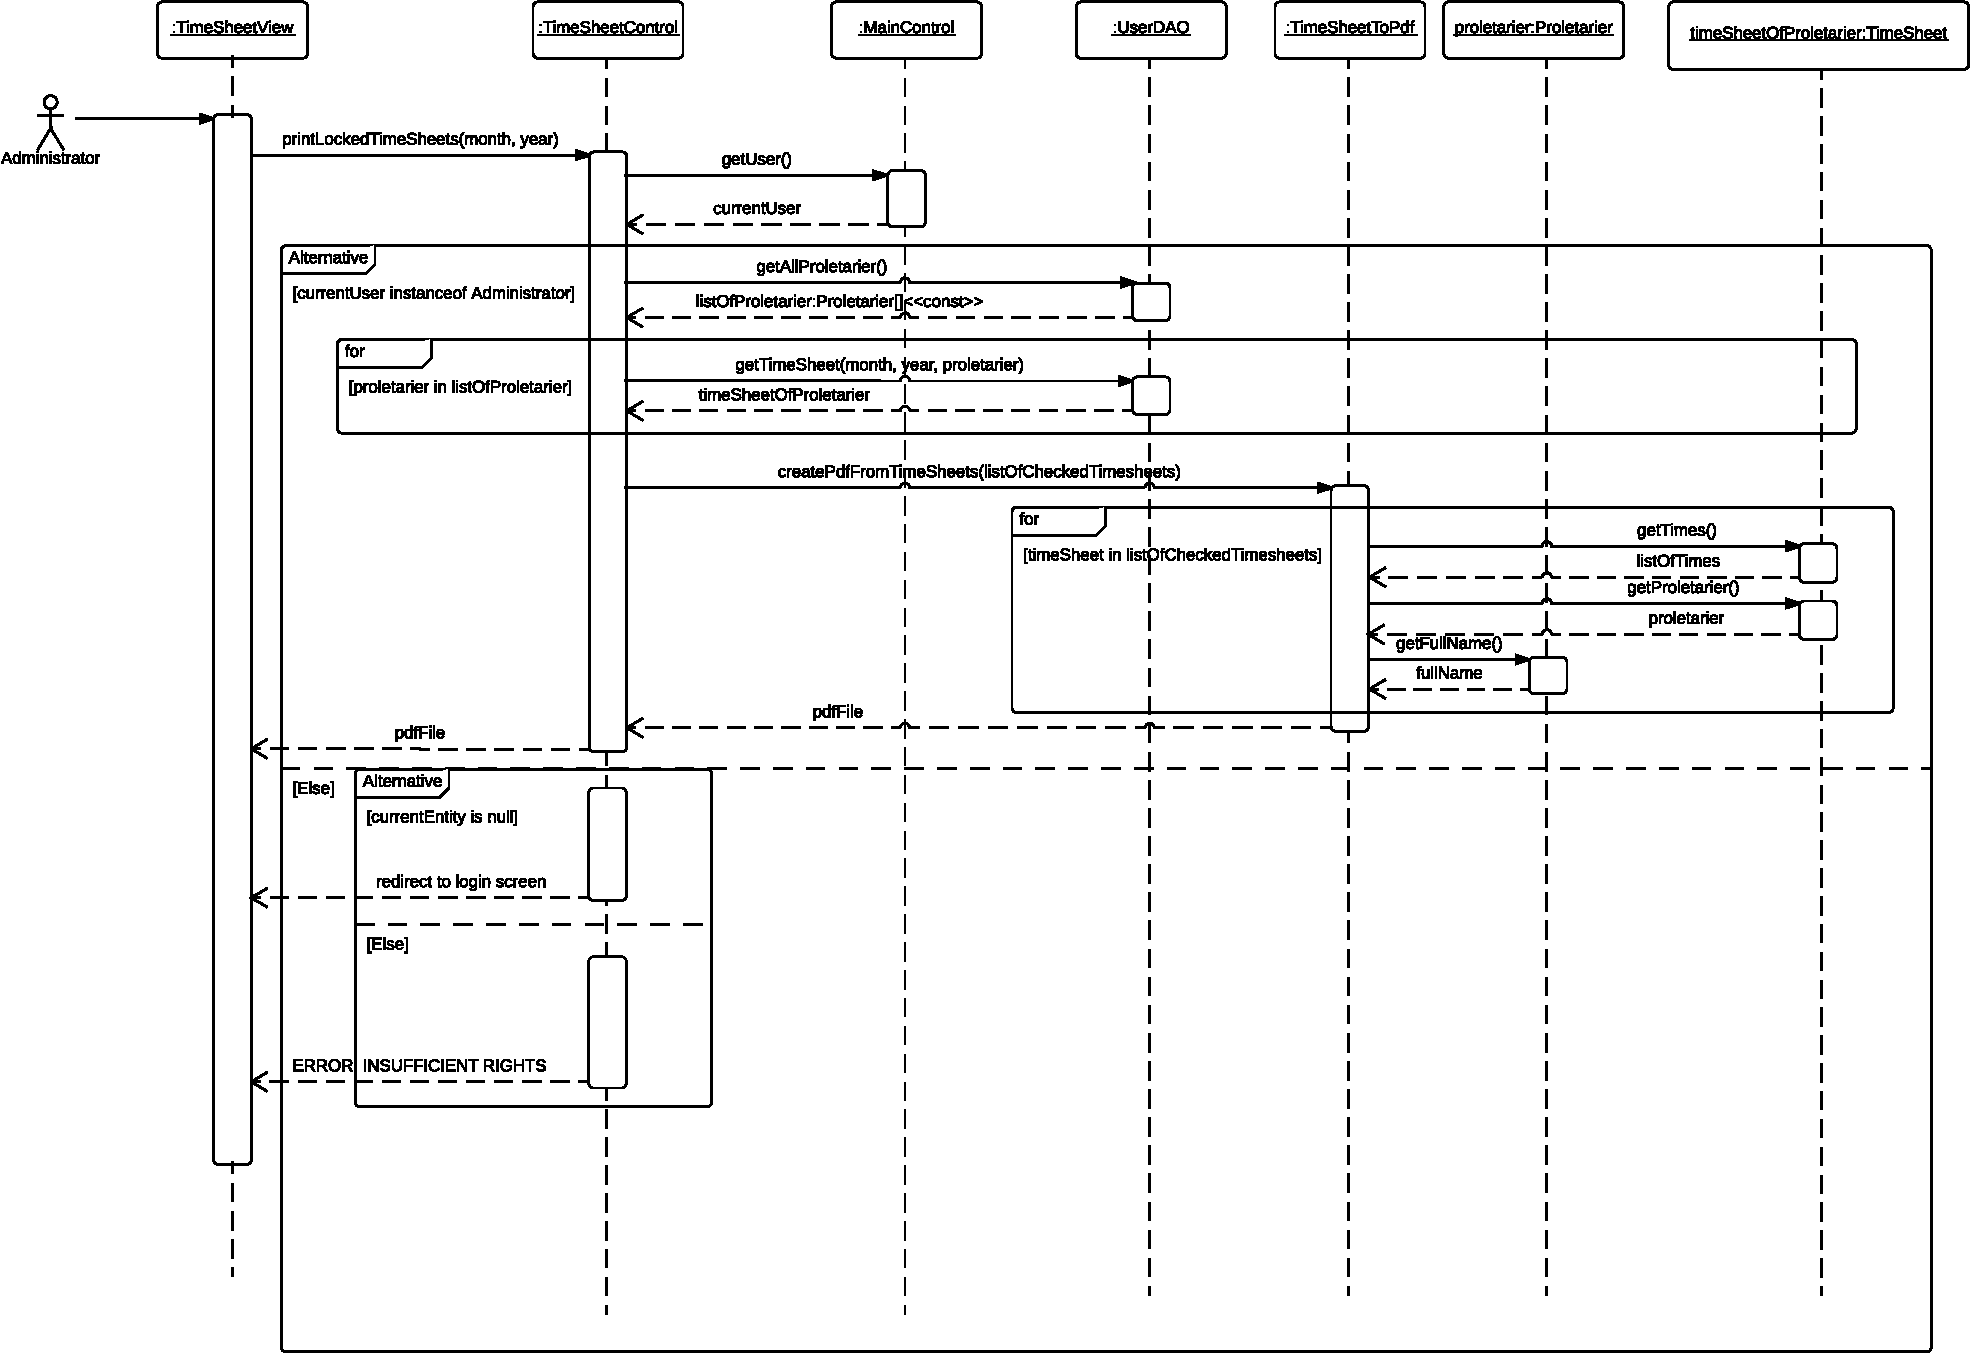
\includegraphics[width=\linewidth]{Diagramms/sequenzes/admin_prints_timesheets.pdf}

    \newpage
    \subsection{Alle Stundenzettel mit Zustand unlocked prüfen}
        Alle Stundenzettel mit dem Zustand unlocked werden auf inkonsistenzen geprüft, zum Beispiel ob der Proletarier gewarnt werden muss, dass der Stundenzettel abgegeben werden muss.\\

        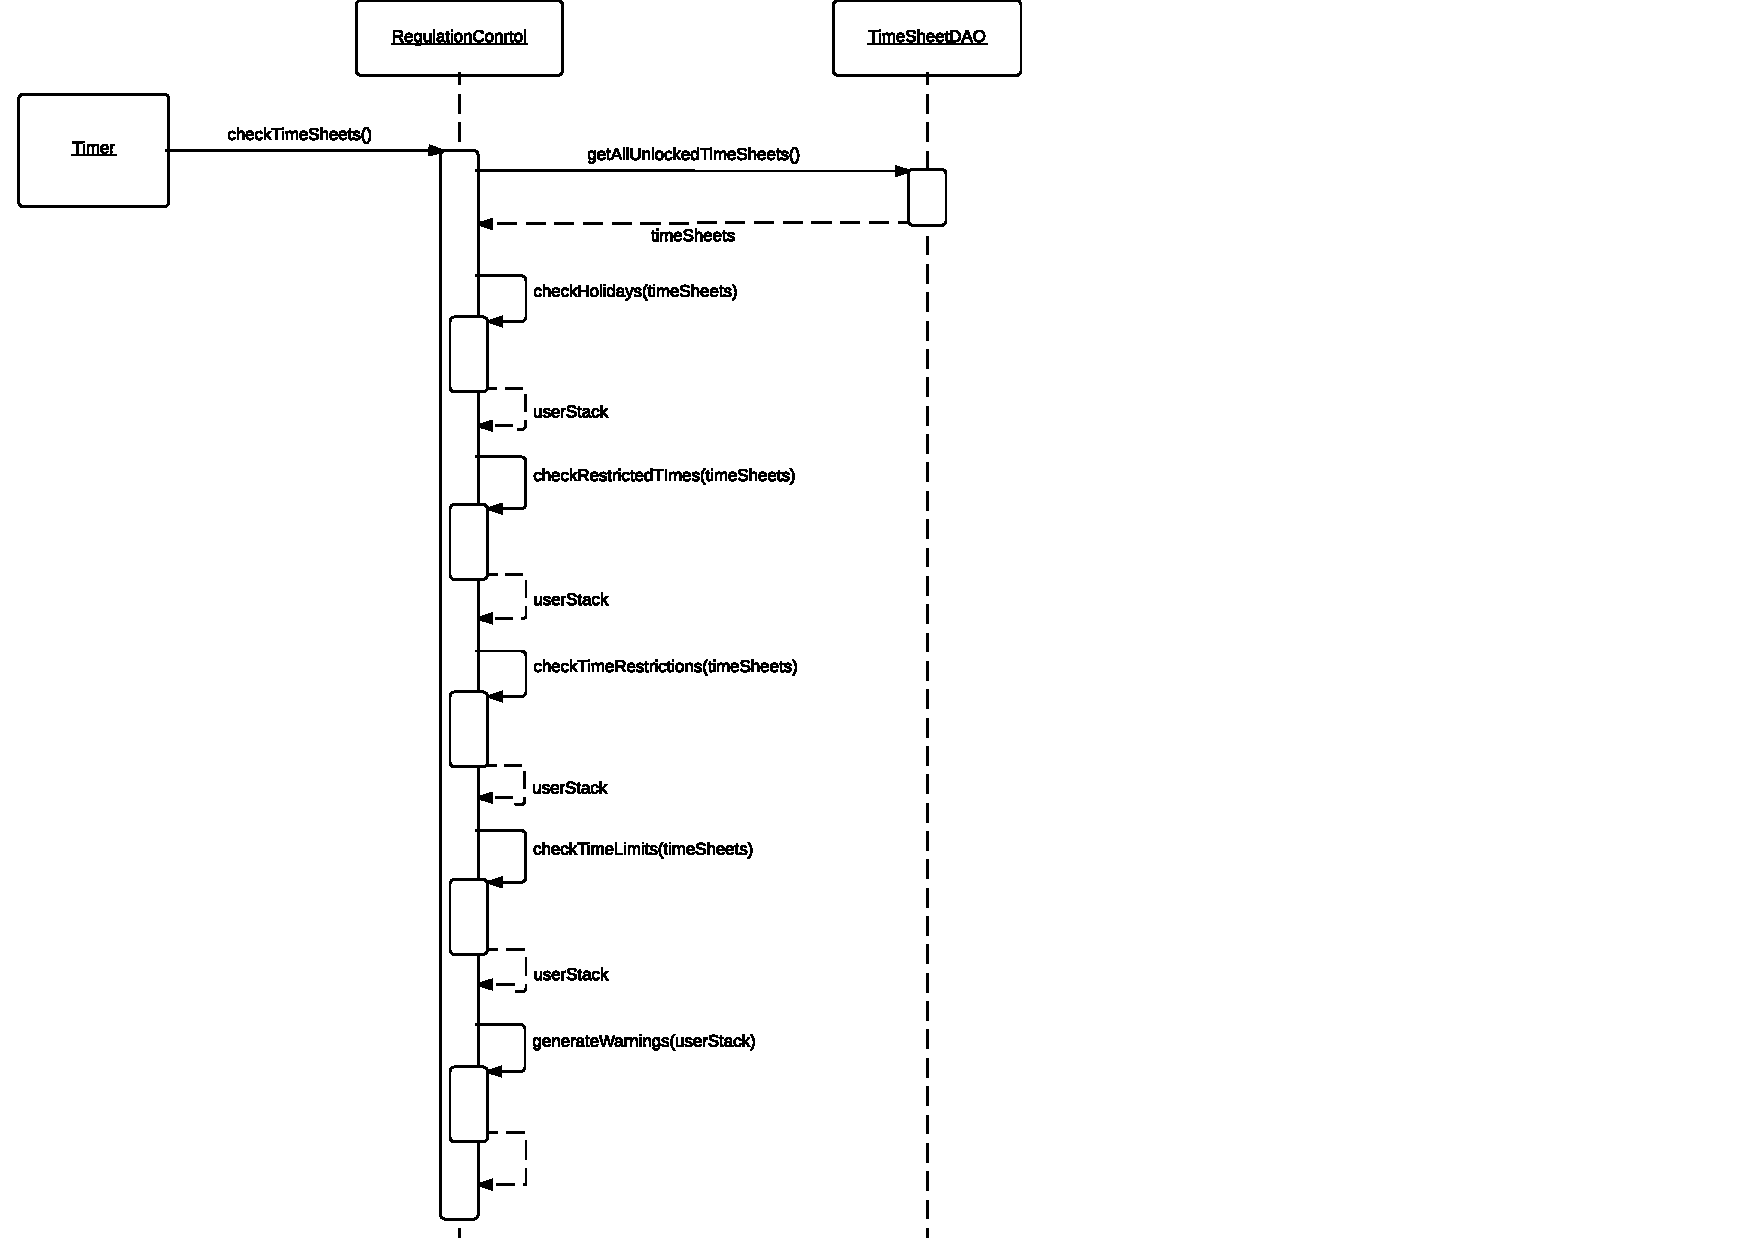
\includegraphics[width=\linewidth]{Diagramms/sequenzes/check_inconsistencies.pdf}

    \newpage
    \subsection{Prüfung eines Stundenzettels auf Rechtskonformität}
        Ein Stundenzettel wird auf Rechtskonformität geprüft.
        Dies beinhaltet die folgenden gesetzlichen Regelungen:
        \begin{itemize}
            \item Die gesetzlich maximale Arbeitszeit wird nicht überschritten (§3 ArbZG).
            \item Die gesetzliche Pausenzeiten werden eingehalten (§4 ArbZG).
            \item Die Ruhezeiten wurden eingehalten (§5 ArbZG).
            \item Es hat keine Nachtarbeit stattgefunden (§6 ArbZG).
            \item Die Sonn- und Feiertagsruhe wurde eingehalten (§9 ArbZG).
                Dabei werden nur die Feiertage in Baden-Württemberg beachtet.
        \end{itemize}

        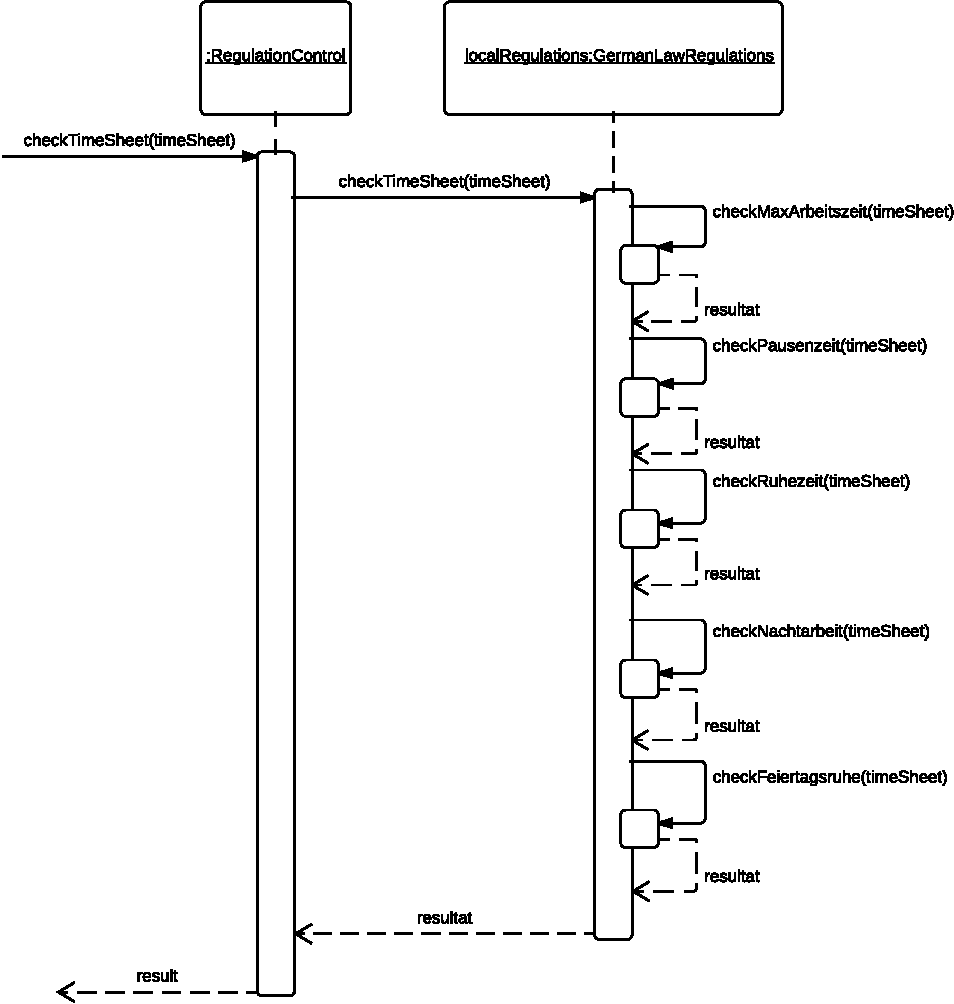
\includegraphics[width=\linewidth-2cm]{Diagramms/sequenzes/check_german_law_regulations.pdf}
